\documentclass[10pt,a4paper]{article}

\usepackage[utf8]{inputenc}
\usepackage[T1]{fontenc}
\usepackage[spanish,es-nodecimaldot]{babel}
\usepackage[top=1.5cm, bottom=2cm, left=1.5cm, right=1.5cm]{geometry}
\usepackage{setspace}
\singlespacing
\usepackage{graphicx}
\usepackage{float}
\usepackage{booktabs}
\usepackage{array}
\usepackage{tabularx}
\usepackage{hyperref}
\usepackage{xcolor}
\usepackage{amsmath}
\usepackage{amssymb}
\usepackage{caption}
\usepackage{subcaption}
\usepackage{listings}
\usepackage{parskip}
\usepackage{csquotes}
\usepackage[backend=biber,style=authoryear,sorting=nyt,maxcitenames=2,maxbibnames=99]{biblatex}
\usepackage{fancyhdr}

\addbibresource{referencias.bib}

\definecolor{codebackground}{HTML}{F5F5F5}
\definecolor{codecomment}{HTML}{6A9955}
\definecolor{codestring}{HTML}{CE9178}
\definecolor{codekeyword}{HTML}{569CD6}
\definecolor{headerdark}{HTML}{2C3E50}

\lstset{
  language=R,
  backgroundcolor=\color{codebackground},
  basicstyle=\ttfamily\footnotesize,
  breaklines=true,
  frame=single,
  rulecolor=\color{gray!40},
  commentstyle=\color{codecomment},
  stringstyle=\color{codestring},
  keywordstyle=\color{codekeyword}\bfseries,
  numbers=left,
  numberstyle=\tiny\color{gray},
  numbersep=5pt,
  tabsize=2,
  showstringspaces=false,
  captionpos=b
}

\hypersetup{
  colorlinks=true,
  linkcolor=headerdark,
  citecolor=headerdark,
  urlcolor=blue!70!black,
  pdftitle={Análisis de Agrupamiento por K-Medias},
  pdfauthor={Juan Muñoz, Vicente Rivera, Fernando Valdés}
}

\captionsetup{font=small, labelfont=bf}

\begin{document}

\begin{center}
  {\LARGE \textbf{Análisis de Agrupamiento por K-Medias}} \\[4pt]
  {\LARGE \textbf{Dataset Paddy -- Metodología CRISP-DM}} \\[10pt]
  {\normalsize Juan Muñoz, Vicente Rivera, Fernando Valdés} \\[2pt]
  {\small juan.munozveloso2023@alu.uct.cl, vrivera2023@alu.uct.cl, fvaldes2023@alu.uct.cl} \\[2pt]
  {\small Tarea 3, INFO1184, Semestre I-2026}
\end{center}

\section*{Resumen}

El presente informe aborda el análisis de segmentación de parcelas de cultivo de arroz (\textit{paddy}) mediante la técnica de agrupamiento por k-medias, siguiendo la metodología CRISP-DM en sus fases de comprensión empresarial, comprensión de los datos, preparación de los datos y modelamiento. El dataset contiene 2.789 registros con 45 variables que describen condiciones agrícolas, climáticas y de rendimiento de parcelas ubicadas en seis bloques agrícolas de la India. Se realizó un análisis exploratorio, preparación de datos con selección de 20 variables numéricas y estandarización \textit{z-score}, y posterior modelamiento con k-medias. Mediante el método del codo y el coeficiente de silueta se determinó $k = 9$ como número óptimo de clusters, obteniendo una silueta promedio de 0,4915 y una razón BSS/TSS de 87,18\%. Los resultados revelan perfiles productivos diferenciados por escala de cultivo, condiciones climáticas regionales y niveles de rendimiento, proporcionando información valiosa para la optimización de prácticas agrícolas. El desarrollo se implementó en el ambiente R Project \parencite{rcore2024}.

\textbf{Palabras clave:} k-medias, CRISP-DM, cultivo de arroz, agrupamiento, segmentación agrícola, R Project.

\section{Introducción}

En el contexto de la inteligencia de negocios aplicada al sector agrícola, la segmentación de parcelas de cultivo constituye una herramienta fundamental para la toma de decisiones sobre siembra, fertilización y riego. La producción de arroz (\textit{paddy}) es un pilar de la seguridad alimentaria global, y la identificación de perfiles productivos permite optimizar recursos, mejorar rendimientos y adaptar estrategias a las condiciones específicas de cada zona.

El presente trabajo utiliza el Paddy Dataset, que contiene registros de parcelas de arroz en seis bloques agrícolas de la India (Cuddalore, Kurinjipadi, Panruti, Kallakurichi, Sankarapuram y Chinnasalem), con información sobre hectáreas, variedades, tipos de suelo, fertilización, condiciones climáticas y rendimiento. El objetivo es aplicar la técnica de agrupamiento por k-medias para descubrir segmentos naturales dentro de las parcelas, siguiendo las primeras cuatro fases de la metodología CRISP-DM \parencite{chapman2000}.

Las preguntas que guían este análisis son: (1) ¿Existen grupos naturales diferenciados entre las parcelas de cultivo? (2) ¿Qué características agrícolas y climáticas definen cada segmento? (3) ¿Cómo pueden estos segmentos informar la planificación agrícola y la asignación de insumos?

\section{Fundamentos de Teoría}

\subsection{Metodología CRISP-DM}

CRISP-DM (\textit{Cross-Industry Standard Process for Data Mining}) es una metodología ampliamente utilizada para estructurar proyectos de minería de datos y analítica \parencite{chapman2000}. Se estructura en seis fases iterativas: (1)~Comprensión empresarial, (2)~Comprensión de los datos, (3)~Preparación de los datos, (4)~Modelamiento, (5)~Evaluación y (6)~Despliegue. Cada fase produce resultados que alimentan a las siguientes, y el proceso permite retroceder a fases previas cuando es necesario, lo que facilita el desarrollo iterativo. En este trabajo se abordan las fases 1 a 4.

\subsection{Agrupamiento por K-Medias}

El algoritmo k-medias es una técnica de aprendizaje no supervisado que particiona un conjunto de $n$ observaciones en $k$ clusters, minimizando la varianza intra-cluster \parencite{macqueen1967,jain2010}. Formalmente, dado un conjunto $\{x_1, x_2, \ldots, x_n\}$, el objetivo es encontrar la partición $S = \{S_1, S_2, \ldots, S_k\}$ que minimice la suma de cuadrados intra-cluster (WSS):

\begin{equation}
  \text{WSS} = \sum_{i=1}^{k} \sum_{x \in S_i} \|x - \mu_i\|^2
\end{equation}

donde $\mu_i$ es el centroide del cluster $S_i$. El algoritmo opera iterativamente: (1)~se inicializan $k$ centroides, (2)~se asigna cada observación al centroide más cercano según la distancia euclidiana, (3)~se recalculan los centroides como la media de las observaciones asignadas, y se repiten los pasos 2--3 hasta convergencia \parencite{hastie2009}.

La distancia euclidiana entre dos puntos $\mathbf{x}$ e $\mathbf{y}$ en $\mathbb{R}^p$ se define como:

\begin{equation}
  d(\mathbf{x}, \mathbf{y}) = \sqrt{\sum_{j=1}^{p}(x_j - y_j)^2}
\end{equation}

\subsection{Validación de Clusters}

Para determinar el número óptimo de clusters se emplean el método del codo, que busca el punto de inflexión en la curva WSS, y el coeficiente de silueta \parencite{rousseeuw1987}. El coeficiente de silueta para una observación $i$ se define como:

\begin{equation}
  s(i) = \frac{b(i) - a(i)}{\max\{a(i), b(i)\}}
\end{equation}

donde $a(i)$ es la distancia media intra-cluster y $b(i)$ la distancia media mínima al cluster más cercano. Un valor cercano a 1 indica buena asignación. La razón BSS/TSS (\textit{Between Sum of Squares} / \textit{Total Sum of Squares}) indica qué proporción de la varianza total es explicada por la separación entre clusters.

\section{Desarrollo del Trabajo}
\subsection{Parte A: Desarrollo con la Metodología CRISP-DM}
\subsubsection{Fase 1: Comprensión Empresarial}

El problema de negocio consiste en optimizar la producción de arroz mediante la identificación de perfiles de parcelas que comparten condiciones agrícolas y climáticas similares. Los productores enfrentan el desafío de asignar insumos (fertilizantes, pesticidas, semillas) de manera eficiente, considerando la variabilidad entre regiones, tipos de suelo y variedades de arroz. Actualmente, las decisiones de gestión agrícola se aplican de forma generalizada sin considerar las particularidades de cada zona productiva, lo que genera ineficiencias en el uso de recursos. Se busca segmentar las parcelas para definir estrategias diferenciadas de gestión agrícola.

El objetivo de minería de datos es descubrir grupos homogéneos de parcelas mediante k-medias, caracterizando cada segmento según variables de escala productiva, fertilización, condiciones climáticas y rendimiento. Siguiendo la terminología CRISP-DM, el criterio de éxito del negocio es mejorar la eficiencia en la asignación de insumos por zona productiva, y el criterio de éxito de minería de datos es obtener clusters con perfiles interpretables y agronómicamente diferenciados \parencite{chapman2000}.

\subsubsection{Fase 2: Comprensión de los Datos}

El dataset \texttt{paddydataset.csv} contiene 2.789 registros y 45 atributos. Las variables se clasifican en: escala de cultivo (\texttt{Hectares}, \texttt{Seedrate}, \texttt{Nursery area}), fertilización (\texttt{DAP}, \texttt{Urea}, \texttt{Potassh}, \texttt{Micronutrients}, \texttt{Pest}), condiciones climáticas (precipitación, temperatura, humedad relativa, viento) y rendimiento (\texttt{Paddy yield}). Las variables categóricas incluyen bloque agrícola (6 niveles), variedad (CO\_43, delux ponni, ponmani), tipo de suelo (aluvial, arcilloso) y tipo de vivero (seco, húmedo). La Tabla~\ref{tab:variables} presenta las variables principales utilizadas en el análisis.

\begin{table}[H]
  \centering
  \caption{Variables principales del dataset Paddy.}
  \label{tab:variables}
  \footnotesize
  \renewcommand{\arraystretch}{1.2}
  \begin{tabularx}{\textwidth}{>{\centering\arraybackslash}p{2.5cm} >{\centering\arraybackslash}p{2cm} >{\centering\arraybackslash}p{3cm} >{\centering\arraybackslash}X}
    \toprule
    \textbf{Variable} & \textbf{Tipo} & \textbf{Rango} & \textbf{Descripción} \\
    \midrule
    Hectares      & Numérica   & 1--6              & Superficie cultivada (Ha) \\
    Paddy yield   & Numérica   & 5.410--38.814     & Rendimiento del cultivo (Kg) \\
    Urea          & Numérica   & 13,6--187,5       & Fertilizante urea a los 40 días (Kg) \\
    DAP           & Numérica   & 6,8--93,8         & Fertilizante DAP a los 20 días (Kg) \\
    Rel. Humidity & Numérica   & 63,3--89,8        & Humedad relativa promedio (\%) \\
    Variety       & Categórica & 3 niveles         & Variedad de arroz cultivada \\
    Soil Types    & Categórica & 2 niveles         & Tipo de suelo (aluvial, arcilloso) \\
    Agri Block    & Categórica & 6 niveles         & Bloque agrícola de ubicación \\
    \bottomrule
  \end{tabularx}
\end{table}

No se detectaron valores faltantes en ninguna variable. El rendimiento medio es de 22.518~Kg (DE~=~9.974~Kg), con un rango de 5.410 a 38.814~Kg, lo que evidencia alta variabilidad productiva. Las hectáreas varían de 1 a 6, y la distribución de variedades es relativamente equilibrada. Las visualizaciones de apoyo para esta fase se presentan en el Anexo (Figuras~\ref{fig:eda_1} a \ref{fig:eda_2}). Del análisis exploratorio se observa que la variedad \textit{delux ponni} presenta los rendimientos más altos, y que existe una fuerte correlación entre las variables de escala (hectáreas, tasa de siembra, fertilizantes). Adicionalmente, la distribución del rendimiento (Figura~\ref{fig:eda_1_dist}) presenta una forma multimodal, lo que sugiere la existencia de subgrupos naturales en los datos, reforzando la pertinencia de aplicar técnicas de agrupamiento.

\subsubsection{Fase 3: Preparación de los Datos}

Para la aplicación de k-medias se realizaron las siguientes transformaciones:

\textbf{Selección de variables:} se eligieron 20 variables numéricas que capturan la escala productiva (hectáreas, tasa de siembra, fertilizante del campo principal), fertilización (DAP, urea, potasio, micronutrientes, pesticida), condiciones climáticas (precipitación e irrigación en cuatro períodos, temperatura mínima y máxima del primer mes, humedad relativa de los dos primeros períodos), residuos (\textit{trash}) y rendimiento final.

\textbf{Estandarización:} se aplicó escalado \textit{z-score} a todas las variables para evitar que aquellas con mayor rango dominen el cálculo de distancias:

\begin{equation}
  z = \frac{x - \bar{x}}{s_x}
\end{equation}

donde $\bar{x}$ es la media y $s_x$ la desviación estándar. Se verificó que las medias resultantes fueran $\approx 0$ y las desviaciones estándar $\approx 1$.

\subsubsection{Fase 4: Modelamiento}

Se aplicó el algoritmo k-medias con 25 inicializaciones aleatorias (\texttt{nstart~=~25}) y semilla fija (42) para reproducibilidad. Se evaluaron valores de $k$ desde 2 hasta 10. El método del codo mostró una disminución gradual del WSS con inflexiones en $k = 4$ y $k = 7$. El coeficiente de silueta promedio alcanzó su máximo en $k = 9$ (0,4915), seguido por $k = 8$ (0,4778) y $k = 7$ (0,4561). Se seleccionó $k = 9$ por maximizar la silueta y ofrecer la mayor separación entre grupos (Fig.~\ref{fig:elbow_sil}).

El modelo final con $k = 9$ obtuvo un WSS total de 7.146,7 y una razón BSS/TSS de 87,18\%, indicando que los clusters explican el 87\% de la varianza total de los datos. La visualización en los dos primeros componentes principales (PCA) muestra una separación clara entre los grupos (Fig.~\ref{fig:clusters_pca}). La evaluación de la asignación final mediante gráfico de silueta se presenta en el Anexo (Figura~\ref{fig:silueta}), donde se aprecia una calidad moderada-buena del agrupamiento.

Los perfiles revelan que los clusters se diferencian principalmente por la escala de cultivo (hectáreas entre 1,4 y 5,2), las condiciones climáticas regionales (temperatura, humedad, precipitación) y el rendimiento resultante (desde 8.138 hasta 31.981~Kg). La Tabla~\ref{tab:perfiles} resume las características de cada cluster. La comparación gráfica de los perfiles por cluster se muestra en la Figura~\ref{fig:perfiles}.

\begin{table}[H]
  \centering
  \caption{Perfiles de los clusters identificados mediante k-medias ($k = 9$).}
  \label{tab:perfiles}
  \footnotesize
  \begin{tabularx}{\textwidth}{c c c c c c X}
    \toprule
    \textbf{Cl.} & \textbf{n} & \textbf{Ha} & \textbf{Yield (Kg)} & \textbf{Urea} & \textbf{Hum. \%} & \textbf{Perfil} \\
    \midrule
    1 & 368 & 4,8 & 29.364 & 129,0 & 72,7 & Escala alta, humedad baja, rendimiento alto \\
    2 & 325 & 3,5 & 21.219 & 96,2  & 86,7 & Escala media, humedad alta, rendimiento medio \\
    3 & 284 & 1,4 & 8.138  & 38,4  & 83,5 & Escala baja, humedad alta, rendimiento bajo \\
    4 & 240 & 4,8 & 29.299 & 129,1 & 78,6 & Escala alta, humedad moderada, rendimiento alto \\
    5 & 365 & 3,6 & 21.246 & 96,3  & 68,1 & Escala media, humedad baja, rendimiento medio \\
    6 & 218 & 1,6 & 9.300  & 43,8  & 68,2 & Escala baja, humedad baja, rendimiento bajo \\
    7 & 325 & 2,5 & 14.634 & 69,1  & 75,1 & Escala media-baja, humedad moderada \\
    8 & 353 & 5,2 & 31.935 & 140,8 & 68,1 & Escala máxima, humedad baja, mayor rendimiento \\
    9 & 311 & 5,2 & 31.981 & 140,8 & 86,7 & Escala máxima, humedad alta, mayor rendimiento \\
    \bottomrule
  \end{tabularx}
\end{table}

\subsubsection{Análisis de Resultados}

El análisis exploratorio permitió identificar alta variabilidad en el rendimiento (5.410 a 38.814~Kg), fuertemente correlacionada con la escala de cultivo. Las variables presentan alta colinealidad entre insumos y hectáreas, lo que justifica la clara separación obtenida por k-medias. Mediante el coeficiente de silueta y el método del codo se seleccionó $k = 9$, obteniendo una silueta promedio de 0,4915 y una razón BSS/TSS de 87,18\%.

La visualización PCA (Fig.~\ref{fig:clusters_pca}) muestra separación clara entre clusters, con los dos primeros componentes principales capturando la mayor parte de la varianza explicada. Los perfiles revelan diferencias relevantes en escala productiva, condiciones climáticas y rendimiento (Tabla~\ref{tab:perfiles} y Fig.~\ref{fig:perfiles}), permitiendo definir segmentos agronómicamente diferenciados. Se observa que los clusters de mayor rendimiento (8 y 9, con $\approx$32.000~Kg) corresponden a parcelas de escala máxima (5,2~Ha), mientras que los de menor rendimiento (3 y 6, con $\approx$8.000--9.000~Kg) corresponden a parcelas pequeñas (1,4--1,6~Ha). La humedad relativa actúa como segundo factor diferenciador, separando clusters de escala similar en función de las condiciones climáticas regionales del bloque agrícola (Fig.~\ref{fig:yield_cluster}).

\subsection{Parte B: Análisis Exploratorio de Datos con Power BI}

Para la parte b) se desarrolló un dashboard en Power BI Desktop con el objetivo de complementar visualmente los hallazgos obtenidos en la metodología CRISP-DM y en el modelamiento con k-medias. El panel fue diseñado para resumir el comportamiento general del dataset y facilitar la interpretación de variables agrícolas, climáticas y de rendimiento en una interfaz orientada a la exploración visual (Figura~\ref{fig:dashboard}).

En una primera etapa se importó el archivo \texttt{paddydataset.csv}. Como parte de la preparación para visualización, se normalizaron los nombres de las columnas, eliminando espacios, paréntesis y sufijos inconsistentes, y adoptando una nomenclatura homogénea orientada a facilitar el modelado, la selección de campos y la legibilidad de las visualizaciones. Posteriormente, se construyeron medidas KPI para rendimiento promedio, rendimiento máximo, rendimiento mínimo, hectáreas totales y tasa de siembra promedio. Estas tarjetas permiten entregar una lectura rápida del contexto general del conjunto de datos, destacando la amplitud del rendimiento observado y su alta variabilidad.

Como visual principal se utilizó un gráfico de dispersión que relaciona la tasa de siembra promedio con el rendimiento promedio por bloque agrícola, usando el tamaño del marcador para representar hectáreas y el color para diferenciar el tipo de suelo. Esta visualización fue priorizada porque permite observar de forma clara una relación positiva entre la intensidad de siembra y el rendimiento, además de mostrar diferencias entre bloques y aportar contexto sobre la escala productiva, lo cual es consistente con los resultados del análisis exploratorio y del clustering.

Se incorporó además un histograma del rendimiento para analizar la distribución de la variable objetivo. Esta visualización resulta relevante porque evidencia concentración de observaciones en determinados rangos y refuerza la existencia de subgrupos en los datos, consistente con la pertinencia del análisis de agrupamiento. Como apoyo interpretativo se añadió una visualización resumida de precipitación por periodo y tipo de suelo, con el fin de incorporar una lectura climática del comportamiento del cultivo. Asimismo, se incluyó un gráfico de dispersión entre urea y rendimiento, utilizado como visual secundaria para explorar si la fertilización reproducía una relación tan marcada como la observada entre tasa de siembra y rendimiento.

Durante el diseño del dashboard se evaluaron otras alternativas gráficas, especialmente comparaciones directas de fertilizantes por bloque agrícola. Sin embargo, esas visualizaciones fueron descartadas como gráficas principales debido a que mostraban un comportamiento muy homogéneo entre bloques y aportaban poca diferenciación analítica. Por ello, se priorizaron gráficos que permitieran observar relaciones con el rendimiento o la forma de su distribución.

En conjunto, el dashboard permitió confirmar visualmente que la tasa de siembra y la escala productiva se asocian de forma positiva con el rendimiento, mientras que las condiciones climáticas aportan contexto complementario para la interpretación de diferencias entre grupos. De esta manera, la Parte B funciona como apoyo exploratorio y comunicacional de los resultados obtenidos en la Parte A.

\section{Discusión y Reflexión}

La metodología CRISP-DM proporcionó un marco estructurado para abordar el análisis de segmentación de parcelas arroceras. Los resultados del k-medias con $k = 9$ evidencian que la variabilidad en el dataset se explica principalmente por dos factores: la escala productiva (hectáreas y las variables de insumos que escalan proporcionalmente) y las condiciones climáticas regionales (humedad relativa y temperatura), que corresponden a los diferentes bloques agrícolas.

La silueta promedio de 0,4915 indica una calidad de agrupamiento moderada-buena, y la razón BSS/TSS de 87,18\% confirma que los clusters capturan la mayor parte de la estructura de los datos. La fuerte correlación entre hectáreas, tasa de siembra y cantidades de fertilizante sugiere que estas variables representan un único factor latente (escala de producción), lo cual explica la claridad de la separación.

Desde la perspectiva agronómica, los clusters de rendimiento alto (8, 9, 1, 4) corresponden a parcelas de mayor escala (4,8--5,2~Ha) con fertilización proporcional, independientemente de las condiciones de humedad. Los clusters de rendimiento bajo (3, 6) corresponden a parcelas pequeñas (1,4--1,6~Ha). El cluster~7 representa un perfil intermedio. Esto sugiere que la escala de producción es el principal determinante del rendimiento absoluto.

Una limitación del análisis es la alta multicolinealidad entre variables de insumos y hectáreas, que podría haberse abordado con reducción de dimensionalidad previa (PCA) o selección más estricta de variables. Como trabajo futuro, se recomienda analizar el rendimiento por hectárea para controlar el efecto de escala, así como incorporar las variables categóricas mediante distancias de Gower.

El dashboard de Power BI reforzó estas conclusiones al evidenciar visualmente las diferencias de rendimiento entre bloques agrícolas y la relación positiva entre escala productiva y rendimiento, facilitando la comunicación de resultados a actores no técnicos del sector agrícola.

\section{Conclusiones}

\textbf{Juan Muñoz:} La aplicación del k-medias con CRISP-DM demostró ser eficaz para identificar 9 segmentos diferenciados en el dataset Paddy, con una silueta de 0,4915 y BSS/TSS del 87,18\%. Los clusters revelan que la escala productiva y las condiciones climáticas regionales son los principales factores de diferenciación entre parcelas, información útil para la planificación agrícola diferenciada.

\textbf{Vicente Rivera:} El análisis exploratorio reveló la ausencia de datos faltantes y una alta variabilidad en el rendimiento (5.410 a 38.814~Kg), fuertemente correlacionada con la escala de cultivo. La estandarización \textit{z-score} fue fundamental para que las variables climáticas, con rangos menores, pudieran contribuir al agrupamiento junto a las variables de producción.

\textbf{Fernando Valdés:} La implementación en R \parencite{rcore2024} permitió un flujo completo desde la exploración hasta la validación. La visualización PCA y el gráfico de silueta confirman la calidad del agrupamiento. Como mejora futura, sería valioso normalizar los insumos y rendimiento por hectárea para detectar eficiencias intrínsecas, lo que permitiría identificar parcelas con alta eficiencia productiva independientemente de su escala.

\printbibliography

\newpage
\section*{Anexo}
\addcontentsline{toc}{section}{Anexo}

\subsection*{A.1 Visualizaciones del Análisis}

\begin{figure}[H]
\centering
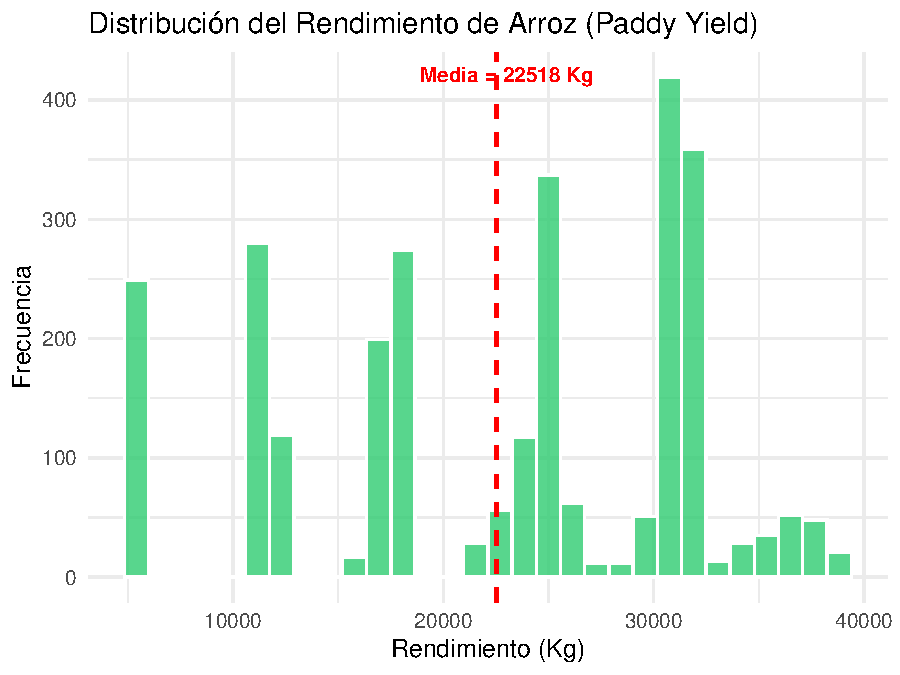
\includegraphics[width=0.9\textwidth]{fig_01_distribucion_yield.pdf}
\caption{Distribución del rendimiento de arroz (Paddy yield).}
\label{fig:eda_1_dist}
\end{figure}

\begin{figure}[H]
\centering
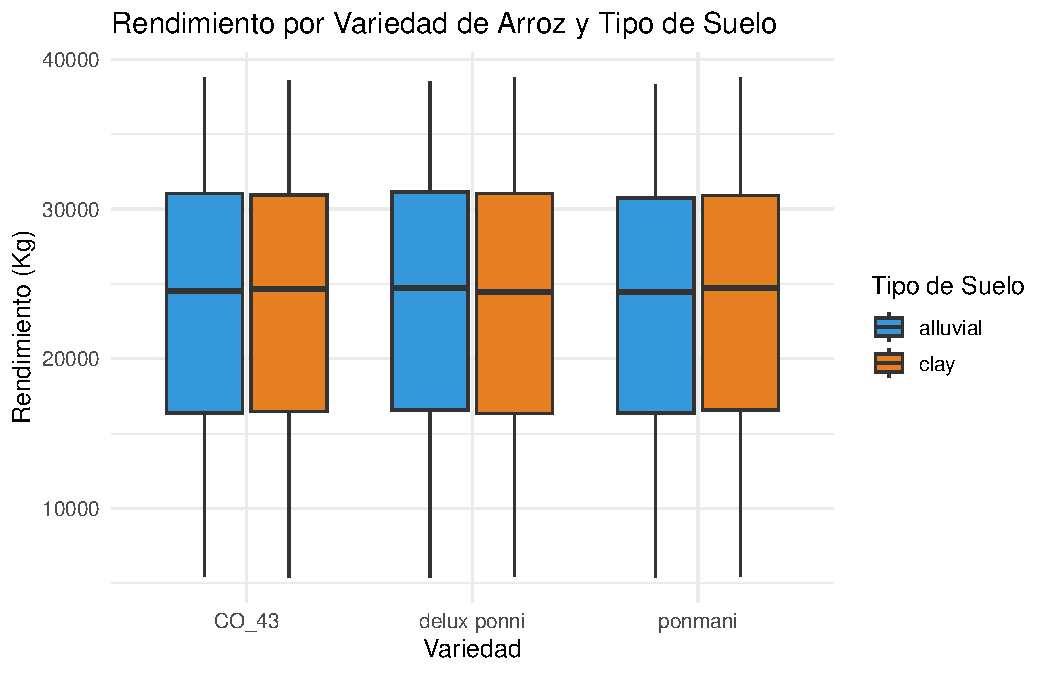
\includegraphics[width=0.9\textwidth]{fig_02_yield_variedad_suelo.pdf}
\caption{Rendimiento por variedad y tipo de suelo.}
\label{fig:eda_1}
\end{figure}

\begin{figure}[H]
\centering
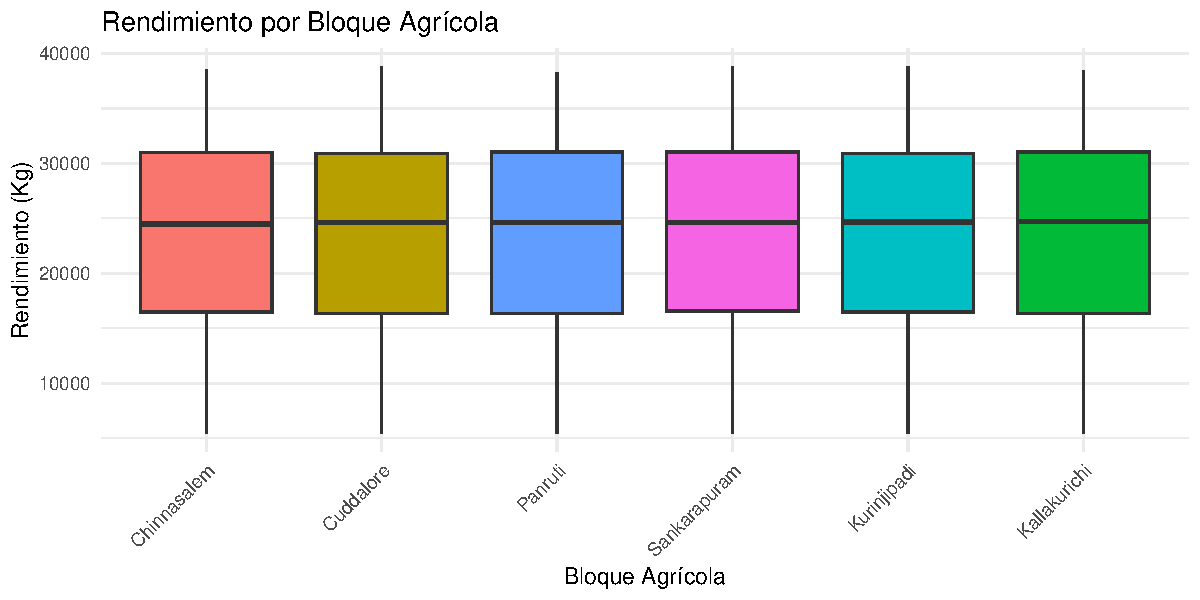
\includegraphics[width=0.9\textwidth]{fig_03_yield_agriblock.pdf}
\caption{Rendimiento por bloque agrícola.}
\label{fig:eda_2_block}
\end{figure}

\begin{figure}[H]
\centering
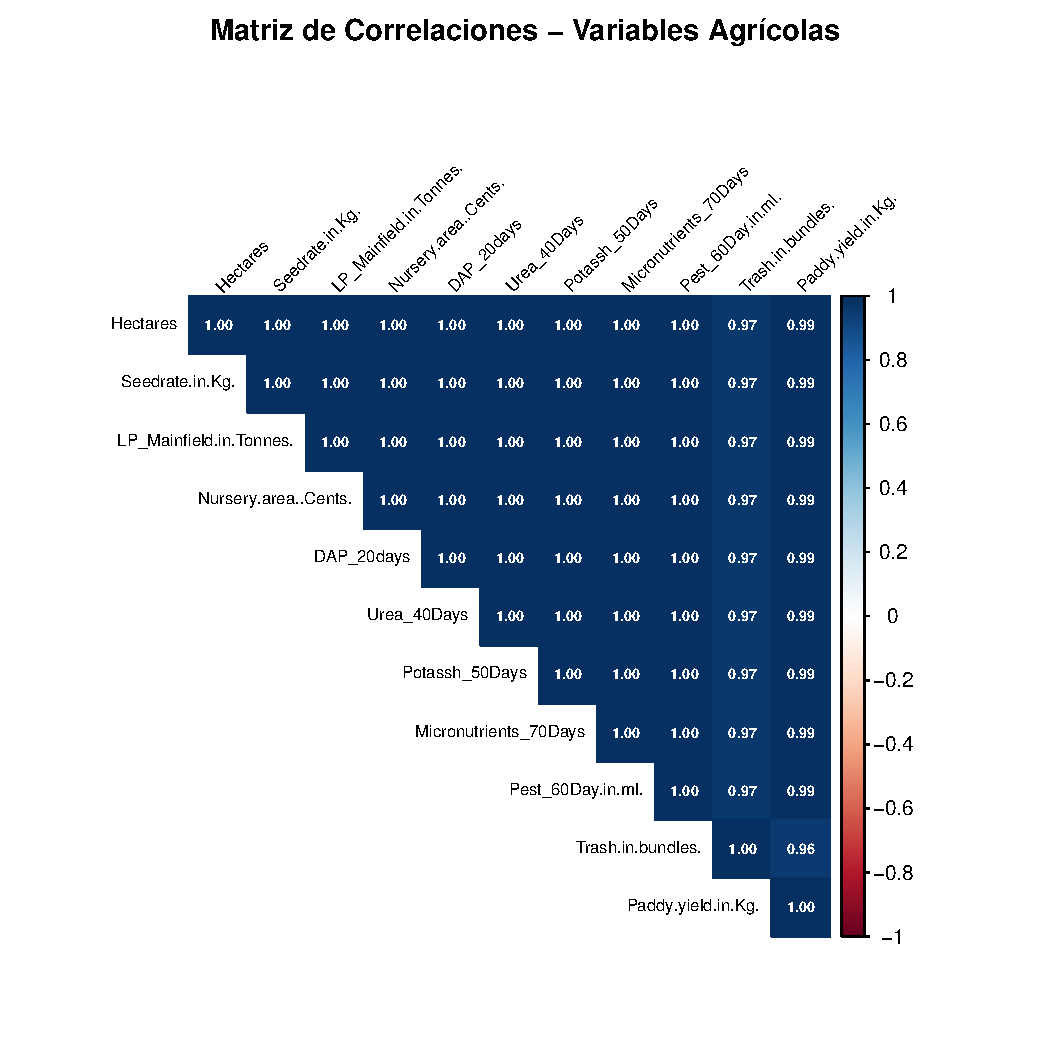
\includegraphics[width=0.55\textwidth]{fig_04_correlaciones.pdf}
\caption{Matriz de correlaciones entre variables numéricas.}
\label{fig:eda_2}
\end{figure}

\begin{figure}[H]
\centering
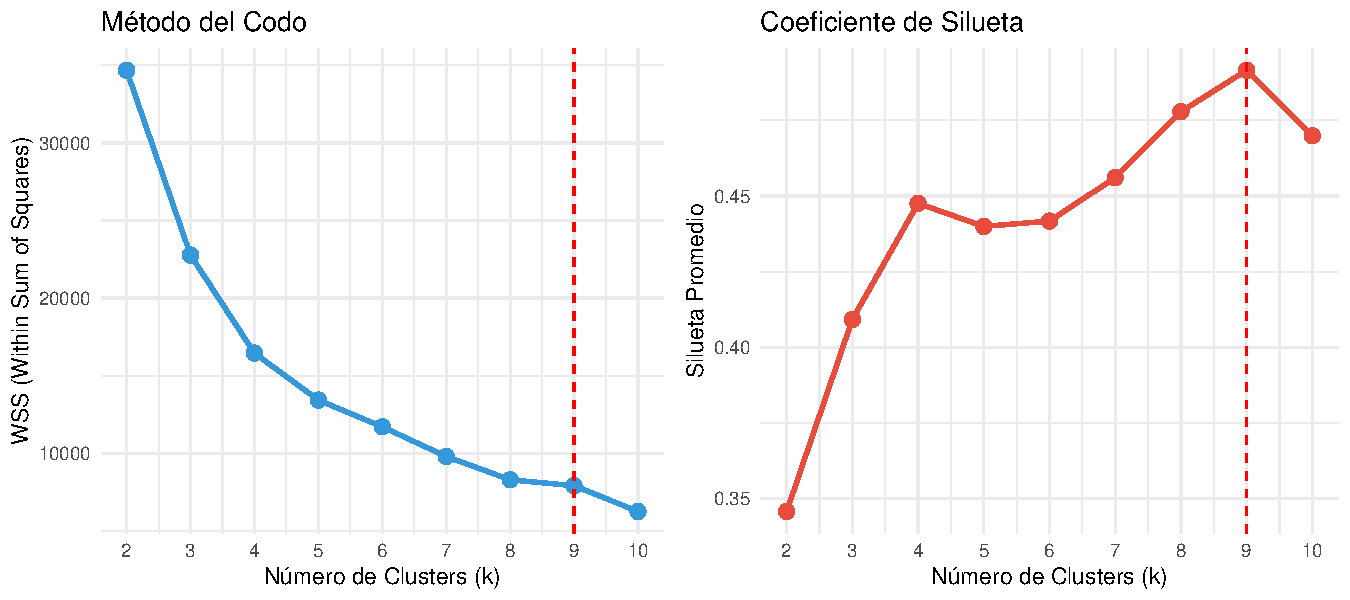
\includegraphics[width=0.85\textwidth]{fig_05_elbow_silhouette.pdf}
\caption{Método del codo (izquierda) y coeficiente de silueta promedio (derecha) para $k = 2$ a $10$.}
\label{fig:elbow_sil}
\end{figure}

\begin{figure}[H]
\centering
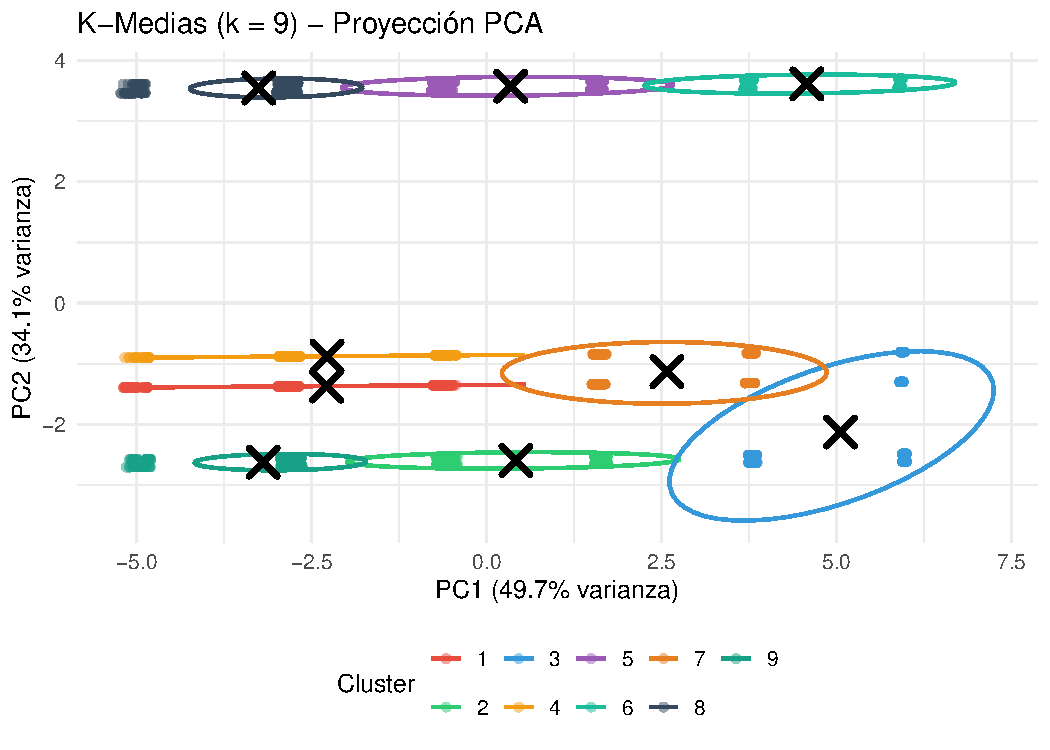
\includegraphics[width=0.9\textwidth]{fig_06_clusters_pca.pdf}
\caption{Clusters proyectados en los dos primeros componentes principales (PCA).}
\label{fig:clusters_pca}
\end{figure}

\begin{figure}[H]
\centering
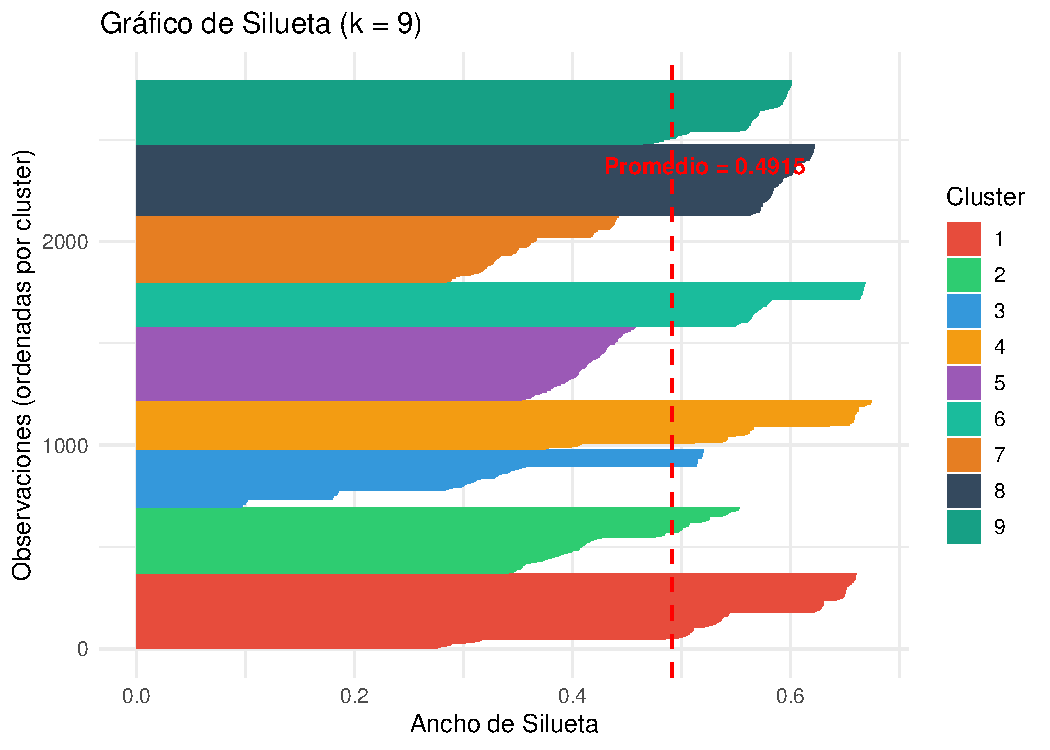
\includegraphics[width=0.55\textwidth]{fig_08_silueta_final.pdf}
\caption{Gráfico de silueta para la asignación final con $k = 9$ clusters.}
\label{fig:silueta}
\end{figure}

\begin{figure}[H]
\centering
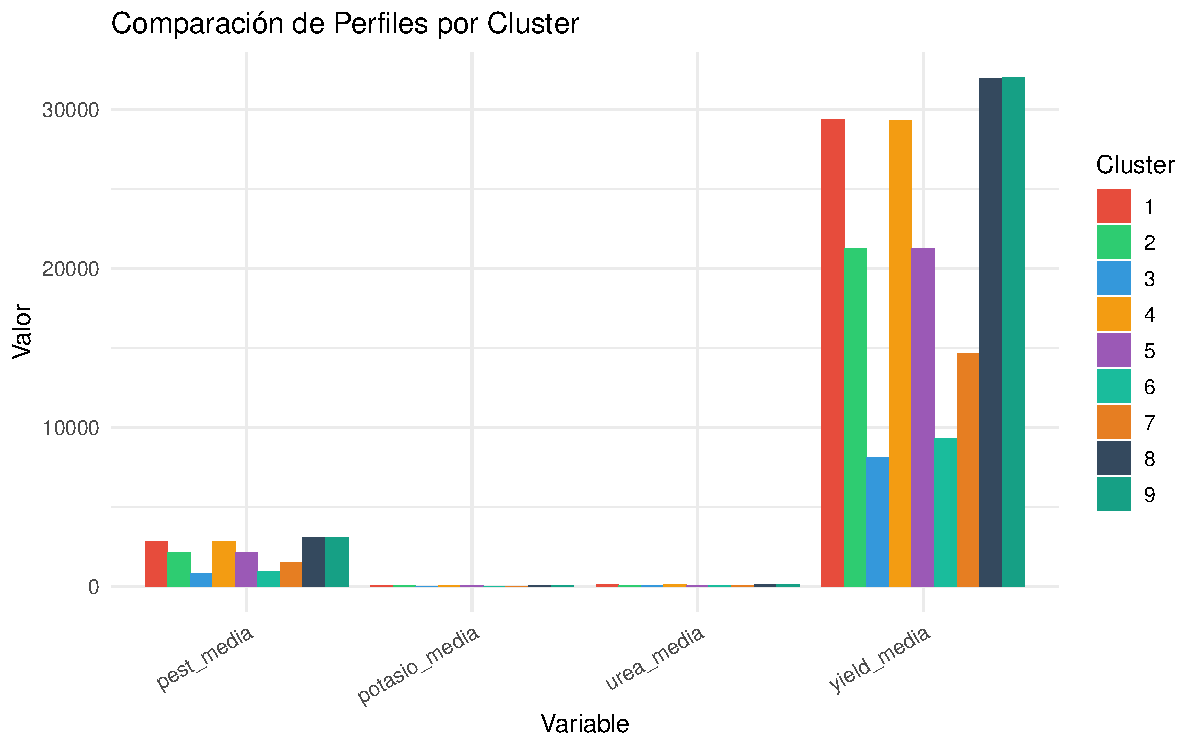
\includegraphics[width=0.85\textwidth]{fig_07_perfiles_clusters.pdf}
\caption{Comparación de perfiles por cluster: variables principales.}
\label{fig:perfiles}
\end{figure}

\begin{figure}[H]
\centering
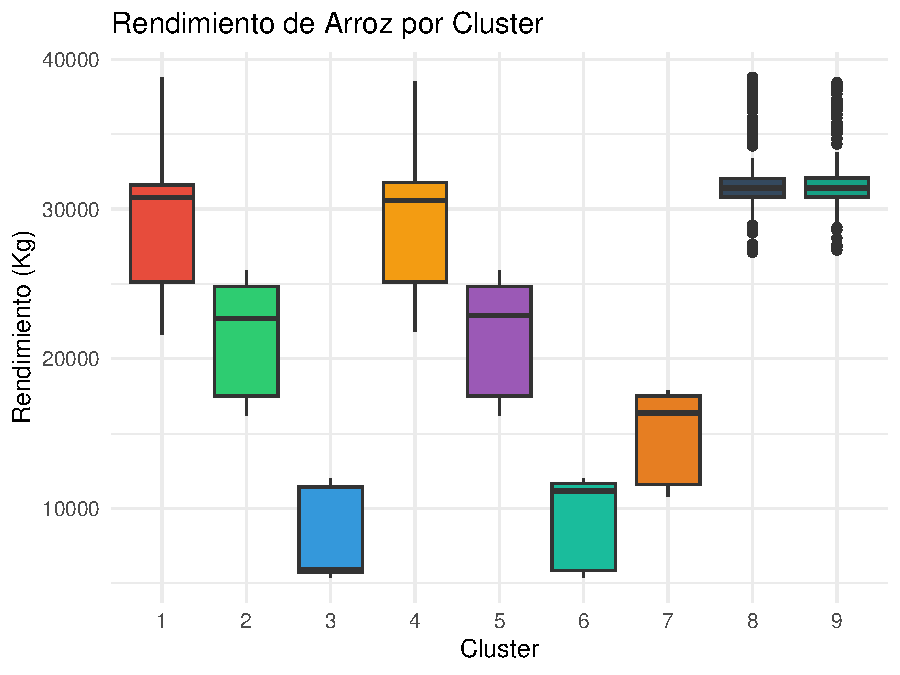
\includegraphics[width=0.85\textwidth]{fig_09_yield_por_cluster.pdf}
\caption{Rendimiento de arroz por cluster.}
\label{fig:yield_cluster}
\end{figure}

\subsection*{A.2 Script R -- Procedimientos Principales}

A continuación se presenta el script principal en R utilizado para el análisis. El código completo se encuentra en el archivo adjunto \texttt{tarea3\_paddy\_kmeans.R}.

\begin{lstlisting}[caption={Carga de datos y análisis exploratorio (Fase 2).}]
# Cargar librerias
library(dplyr)
library(ggplot2)
library(cluster)
library(corrplot)
library(tidyr)
library(gridExtra)

# Cargar datos
paddy <- read.csv("dataset/paddydataset.csv",
                   stringsAsFactors = TRUE)
cat("Dimensiones:", dim(paddy), "\n")
summary(paddy)

# Distribucion de rendimiento
ggplot(paddy, aes(x = Paddy.yield.in.Kg.)) +
  geom_histogram(bins = 30, fill = "#2ecc71") +
  labs(title = "Distribucion del Rendimiento",
       x = "Rendimiento (Kg)", y = "Frecuencia") +
  theme_minimal()

# Rendimiento por variedad y suelo
ggplot(paddy, aes(x = Variety, y = Paddy.yield.in.Kg.,
                  fill = Soil.Types)) +
  geom_boxplot() +
  labs(title = "Rendimiento por Variedad y Suelo") +
  theme_minimal()
\end{lstlisting}

\begin{lstlisting}[caption={Preparación de datos y estandarización (Fase 3).}]
# Seleccion de 20 variables numericas
paddy_prep <- paddy %>%
  select(Hectares, Seedrate.in.Kg.,
    LP_Mainfield.in.Tonnes., DAP_20days,
    Urea_40Days, Potassh_50Days,
    Micronutrients_70Days, Pest_60Day.in.ml.,
    X30DRain..in.mm., X30DAI.in.mm.,
    X30_50DRain..in.mm., X30_50DAI.in.mm.,
    X51_70DRain.in.mm., X51_70AI.in.mm.,
    Min.temp_D1_D30, Max.temp_D1_D30,
    Relative.Humidity_D1_D30,
    Relative.Humidity_D31_D60,
    Trash.in.bundles., Paddy.yield.in.Kg.)

# Estandarizacion z-score
paddy_scaled <- scale(paddy_prep)
\end{lstlisting}

\begin{lstlisting}[caption={Modelado: K-medias y validación (Fase 4).}]
# Metodo del codo y silueta para k = 2..10
set.seed(42)
wss <- sapply(2:10, function(k) {
  km <- kmeans(paddy_scaled, centers = k,
               nstart = 25, iter.max = 100)
  km$tot.withinss
})
avg_sil <- sapply(2:10, function(k) {
  set.seed(42)
  km <- kmeans(paddy_scaled, centers = k,
               nstart = 25, iter.max = 100)
  mean(silhouette(km$cluster,
       dist(paddy_scaled))[, 3])
})

# K-Medias final con k optimo
k_opt <- which.max(avg_sil) + 1  # k = 9
km_final <- kmeans(paddy_scaled, centers = k_opt,
                   nstart = 25, iter.max = 100)
cat("BSS/TSS:", km_final$betweenss /
    km_final$totss * 100, "%\n")

# Visualizacion PCA
pca_result <- prcomp(paddy_scaled)
pca_df <- data.frame(PC1 = pca_result$x[,1],
  PC2 = pca_result$x[,2],
  Cluster = as.factor(km_final$cluster))
ggplot(pca_df, aes(x=PC1, y=PC2, color=Cluster)) +
  geom_point(alpha=0.5) +
  stat_ellipse(level=0.90) +
  theme_minimal()

# Silueta final
sil <- silhouette(km_final$cluster,
                  dist(paddy_scaled))
cat("Silueta promedio:", mean(sil[,3]), "\n")
\end{lstlisting}

\subsection*{A.3 Parte b) -- Dashboard en Power BI}

El dashboard construido en Power BI Desktop incluye las siguientes visualizaciones: (1) tarjetas KPI con rendimiento promedio, rendimiento máximo, rendimiento mínimo, hectáreas totales y tasa de siembra promedio; (2) gráfico de dispersión principal de tasa de siembra vs.\ rendimiento por bloque agrícola, con tamaño por hectáreas y color por tipo de suelo; (3) histograma de la distribución del rendimiento; (4) gráfico de precipitación por periodo y tipo de suelo; y (5) gráfico de dispersión secundario de urea vs.\ rendimiento. El archivo \texttt{.pbix} se adjunta como evidencia del dashboard.

\begin{figure}[H]
\centering
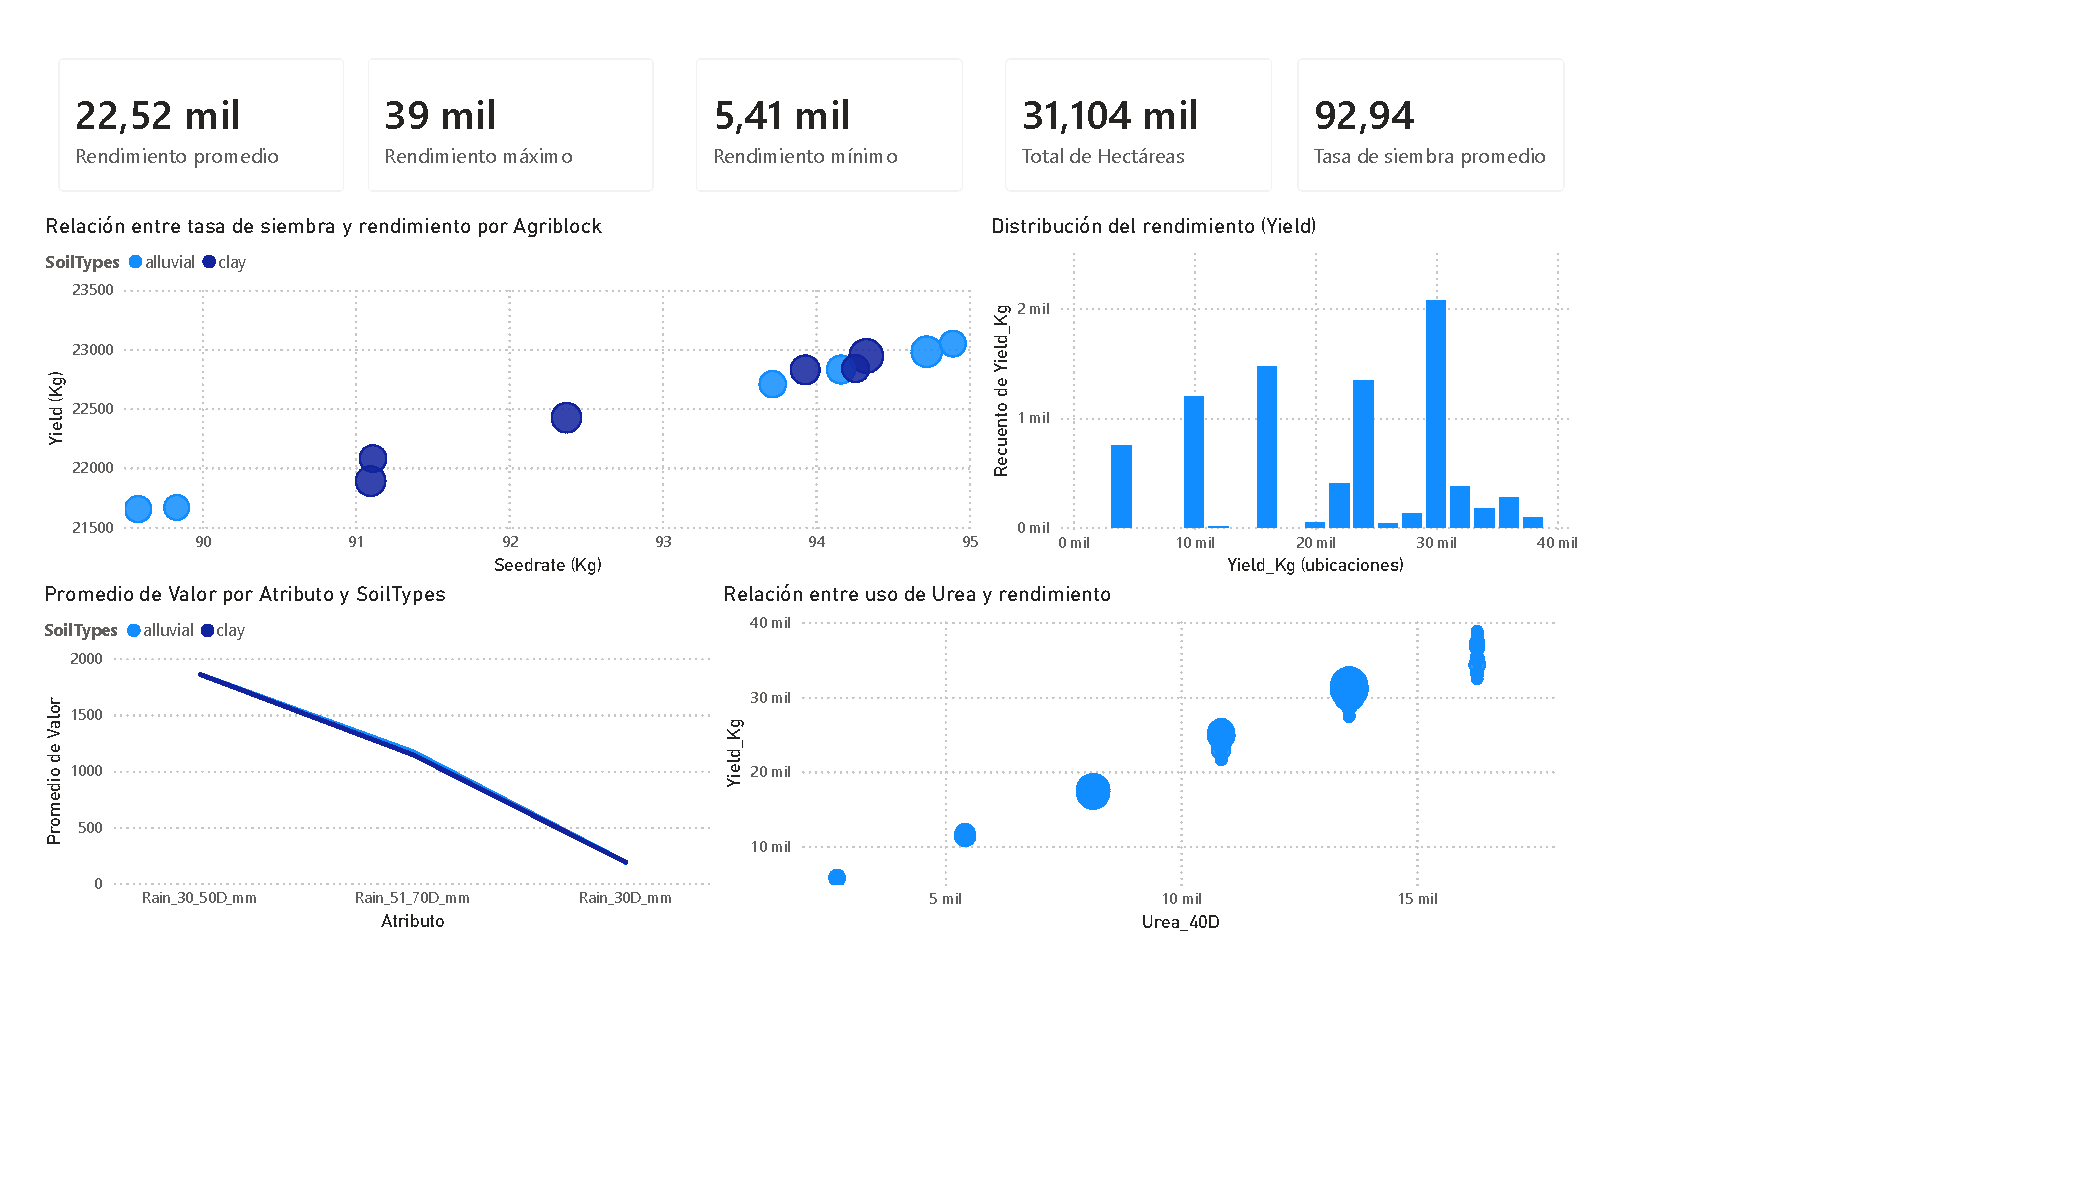
\includegraphics[width=1\textwidth]{dashboard.pdf}
\caption{Dashboard de Power BI utilizado para el análisis exploratorio del dataset Paddy.}
\label{fig:dashboard}
\end{figure}

\subsection*{A.4 Bitácora de Trabajo}

\begin{table}[H]
  \centering
  \footnotesize
  \caption{Bitácora de trabajo grupal.}
  \label{tab:bitacora}
  \begin{tabularx}{\textwidth}{l X l}
    \toprule
    \textbf{Fecha} & \textbf{Actividad} & \textbf{Responsable} \\
    \midrule
    11-04-2026 & Comprensión empresarial: definición del problema de segmentación de parcelas arroceras, identificación de objetivos de minería de datos y revisión bibliográfica sobre k-medias y CRISP-DM. Descarga y lectura inicial del dataset Paddy (2.789 registros, 45 variables). & Todos \\
    11-04-2026 & Análisis exploratorio de datos (Fase~2): estadísticas descriptivas con \texttt{summary()}, distribución del rendimiento, visualización de relaciones entre rendimiento, variedad, tipo de suelo y bloque agrícola. Generación de la matriz de correlaciones entre variables numéricas. & Juan Muñoz \\
    12-04-2026 & Preparación de datos (Fase~3): selección de 20 variables numéricas relevantes, verificación de ausencia de datos faltantes, estandarización \textit{z-score} con \texttt{scale()} y validación de medias $\approx 0$ y desviaciones estándar $\approx 1$. & Fernando Valdés \\
    12-04-2026 & Modelamiento (Fase~4): implementación de k-medias con 25 inicializaciones (\texttt{nstart~=~25}), evaluación de $k = 2$ a $10$ mediante método del codo y coeficiente de silueta, selección de $k = 9$, visualización PCA y gráfico de silueta final. & Juan Muñoz \\
    13-04-2026 & Construcción del dashboard en Power BI Desktop: importación del dataset, normalización de nombres de columnas, creación de tarjetas KPI, gráfico de dispersión tasa de siembra vs.\ rendimiento por bloque agrícola, histograma de rendimiento, gráfico de precipitación por periodo y tipo de suelo, y dispersión urea vs.\ rendimiento. & Vicente Rivera \\
    13-04-2026 & Análisis e interpretación de resultados: caracterización de los 9 clusters, elaboración de la tabla de perfiles, análisis de la razón BSS/TSS (87,18\%) y discusión de las implicancias agronómicas de cada segmento. & Todos \\
    14/15-04-2026 & Redacción del informe en \LaTeX{}, integración de figuras y tablas, redacción de fundamentos teóricos, discusión, reflexión y conclusiones individuales. Revisión cruzada del documento y entrega final. & Todos \\
    \bottomrule
  \end{tabularx}
\end{table}

\end{document}
